\documentclass[a4paper]{article}

%% Language and font encodings
\usepackage[english]{babel}
\usepackage[utf8x]{inputenc}

\usepackage[T1]{fontenc}
\usepackage{wrapfig, blindtext}

%% Sets page size and margins
\usepackage[a4paper,top=3cm,bottom=2cm,left=3cm,right=3cm,marginparwidth=1.75cm]{geometry}

%% Useful packages
\usepackage{amsmath}
\usepackage{graphicx}
\usepackage[colorinlistoftodos]{todonotes}
%Color a las referencias
\usepackage[colorlinks=true, allcolors=blue]{hyperref}
%Color a los textos

%Caratula
\begin{document}
\begin{titlepage}
\begin{center}
\vspace*{-0.4in}

{\fontsize{12}{30}\bf \selectfont UNIVERSIDAD NACIONAL DE INGENIERIA\\}

{\fontsize{12}{40}\bf \selectfont FACULTAD DE CIENCIAS\\}
\vspace*{0.15in} CIENCIAS DE LA COMPUTACI\'ON\\
\vspace*{0.2in}


\begin{center}

\includegraphics[width=5cm,height=6.5cm]{UNI.png}
\end{center}
\vspace*{0.2in}

\begin{large}
	{\bf PROYECTO DE BIOLOGIA COMPUTACIONAL\\}
	\vspace*{0.3in}
\end{large}

\begin{large}
{\bf T\'itulo del Trabajo\\}
\vspace*{0.2in}
\end{large}

\begin{Large}
\color{blue}
\textbf{GATTACA\\}
\color{black}
\end{Large}
\vspace*{0.2in}

\begin{large}
{\bf Autores} 
\vspace*{0.1in}
\\L\'azaro Camasca, Edson Nicks\\
Leon Rios, Marco Naro
\end{large}
\vspace*{0.4in}


\begin{large}
{\bf Profesor} 
\vspace*{0.1in}
\\Nuñez Iturri, Ciro Javier
\end{large}

\end{center}
\begin{center}
\begin{large}
\vspace*{1.0in}
Lima - Peru\\
{\bf (2019)}
\end{large}
\end{center}
\end{titlepage}

\pagebreak
\tableofcontents
\pagebreak

\section{Objetivos}

\subsection{Objetivos Generales}
\begin{itemize}
\item Creación de un aplicación gráfica usando BioPython y TKinter para el analisis de información Genética de Especies endémicas de las regiones del Perú.

\end{itemize}

\subsection{Objetivos Específicos}

\begin{itemize}
\item Recolectar información genética de especies endémicas.
\item Desarrollar la aplicación para el análisis de secuencias,.
\item Desarrollar algoritmos para obtener las alineaciones, árboles filogenéticos 
\item Evaluar el árbol filogenético
\end{itemize}

\section{Resumen Ejecutivo}

Se pretender crear una aplicación gráfica conectada a una base de datos con la información genética de las especies endémicas del Perú, el software procesara las secuencias, creará el árbol filogenético, mostrará los resultados y analizará las relaciones evolutivas de las especies escogidas.
Se escogió como marcaadores moleculares a la proteína NADH deshidrogenasa subunidad 2 debido la importante \textbf{función respiratoria mitocondrial}, hecho por el cual tiene presencia en todas las especies escogidas.
Se realizó el alineamiento utilizando software Clustal Omega.
Se utilizó el modelo evolutivo Kimura y el método para la construcción de árbol escogido fue un método basado en agrupamiento, de los cuales se implemento el método UPGMA y el método Unión de vecinos(NJ).

\section{Descripción del Proyecto}

El proyecto esta implementado netamente en el lenguaje Python
Las librerías utilizadas serán:
\begin{itemize}
\item BioPython para el procesamiento de secuencias
\item Tkinter para el entorno gráfico.

\end{itemize}

\noindent El software incluye:
\begin{itemize}

\item Dentro de la GUI, se pobre escoger las especies para el análisis posterior.
\item Datos reales recolectados de la base de datos de NCBI.
\item Algoritmos implementados para el alineamiento de Genes homólogos.
\item Algoritmos implementados para el alineamiento de Proteínas.
\item Algoritmos para la Generación de Arboles Filogenéticos.

\end{itemize}

\noindent La \textbf{metodología} que se implanto para el desarrollo del proyecto es el siguiente:

\subsection{Determinar las especies y el material a utilizar}

Las especies se escogieron fueron especies endémicas del Perú, especias en \textbf{peligro de extinción} en el Perú y \textbf{especies representativas} del Perú. Además, se tuvo en cuenta la disponibilidad de material genético puesto que muchas de las especies endémicas poseen una base de datos genética incompleta y algunas no se encuentran codificadas en absoluto.\\

\noindent El material genetico se encuentran en la base de datos de NCBI, los nombres son un enlace para poder optener más información en NCBI.\\

\noindent Se escogió las siguientes 11 especies:
\begin{itemize}
    \item \href{https://www.ncbi.nlm.nih.gov/protein/ABM63279.1/}{\underline{Tremarctos ornatus}}
    
    \item 
    \href{https://www.ncbi.nlm.nih.gov/protein/AIY56286.1}{\underline{Panthera onca}}
    
    \item 
    \href{https://www.ncbi.nlm.nih.gov/protein/ACJ45788.1}{\underline{Vicugna vicugna}}
    
    \item 
    \href{https://www.ncbi.nlm.nih.gov/protein/329756060}{\underline{Aulacorhynchus huallagae}}
    
    \item 
    \href{https://www.ncbi.nlm.nih.gov/protein/YP_009178568.1}{\underline{Leopardus jacobita}}
    
    \item 
    \href{https://www.ncbi.nlm.nih.gov/protein/NP_944712.1}{\underline{Inia geoffrensis}}
    
    \item 
    \href{https://www.ncbi.nlm.nih.gov/protein/AON77377.1}{\underline{Spheniscus humboldti}}
    
    \item 
    \href{https://www.ncbi.nlm.nih.gov/protein/AEH42425.1}{\underline{Vultur gryphus}}
    
    \item 
    \href{https://www.ncbi.nlm.nih.gov/protein/BAH23368.1}{\underline{Lama glama}}
    
    \item 
    \href{https://www.ncbi.nlm.nih.gov/protein/AJE26518.1}{\underline{Cavia porcellus}}
    
    \item 
    \href{https://www.ncbi.nlm.nih.gov/protein/298371651}{\underline{Platalea ajaja}}
    
\end{itemize}


\subsection{Elegir los marcadores moleculares}
La elección de los marcadores moleculares es una parte importante porque puede hacer una \textbf{gran diferencia} en la
obtención de un árbol correcto.

\noindent Entre los marcadores moleculares, secuencias de nucleótidos o de proteínas, se optó por utilizar \textbf{secuencias de proteínas} por las siguientes razones:


\begin{itemize}
	\item Como se va estudiar la evolución de grupos de \textbf{organismos ampliamente divergentes} se aconseja utilizar secuencias de proteínas.
	\item Las relaciones filogenéticas que se están analizando están en el \textbf{nivel más profundo - bacteriana}, por ello lo más adecuado es usar secuencias de proteínas conservadas.
\end{itemize}


\subsubsection{Proteina NADH deshidrogenasa}

La proteína a analizarse sera el NADH deshidrogenasa, también conocido como Complejo I, subunidad 2 debido a que se encuentra presente en todas las especias y está codificado. \\
La proteína escogida cumple una importante \textbf{función en la respiración bacteriana y mitocondrial}. Por ende, es posible encontrarla en diversas especies y no es extraño que se haya codificado.\\
Una importante observación es que no todas las especies se encuentran codificadas en la base de datos de NCBI, faltando genes importantes.

\begin{center}
	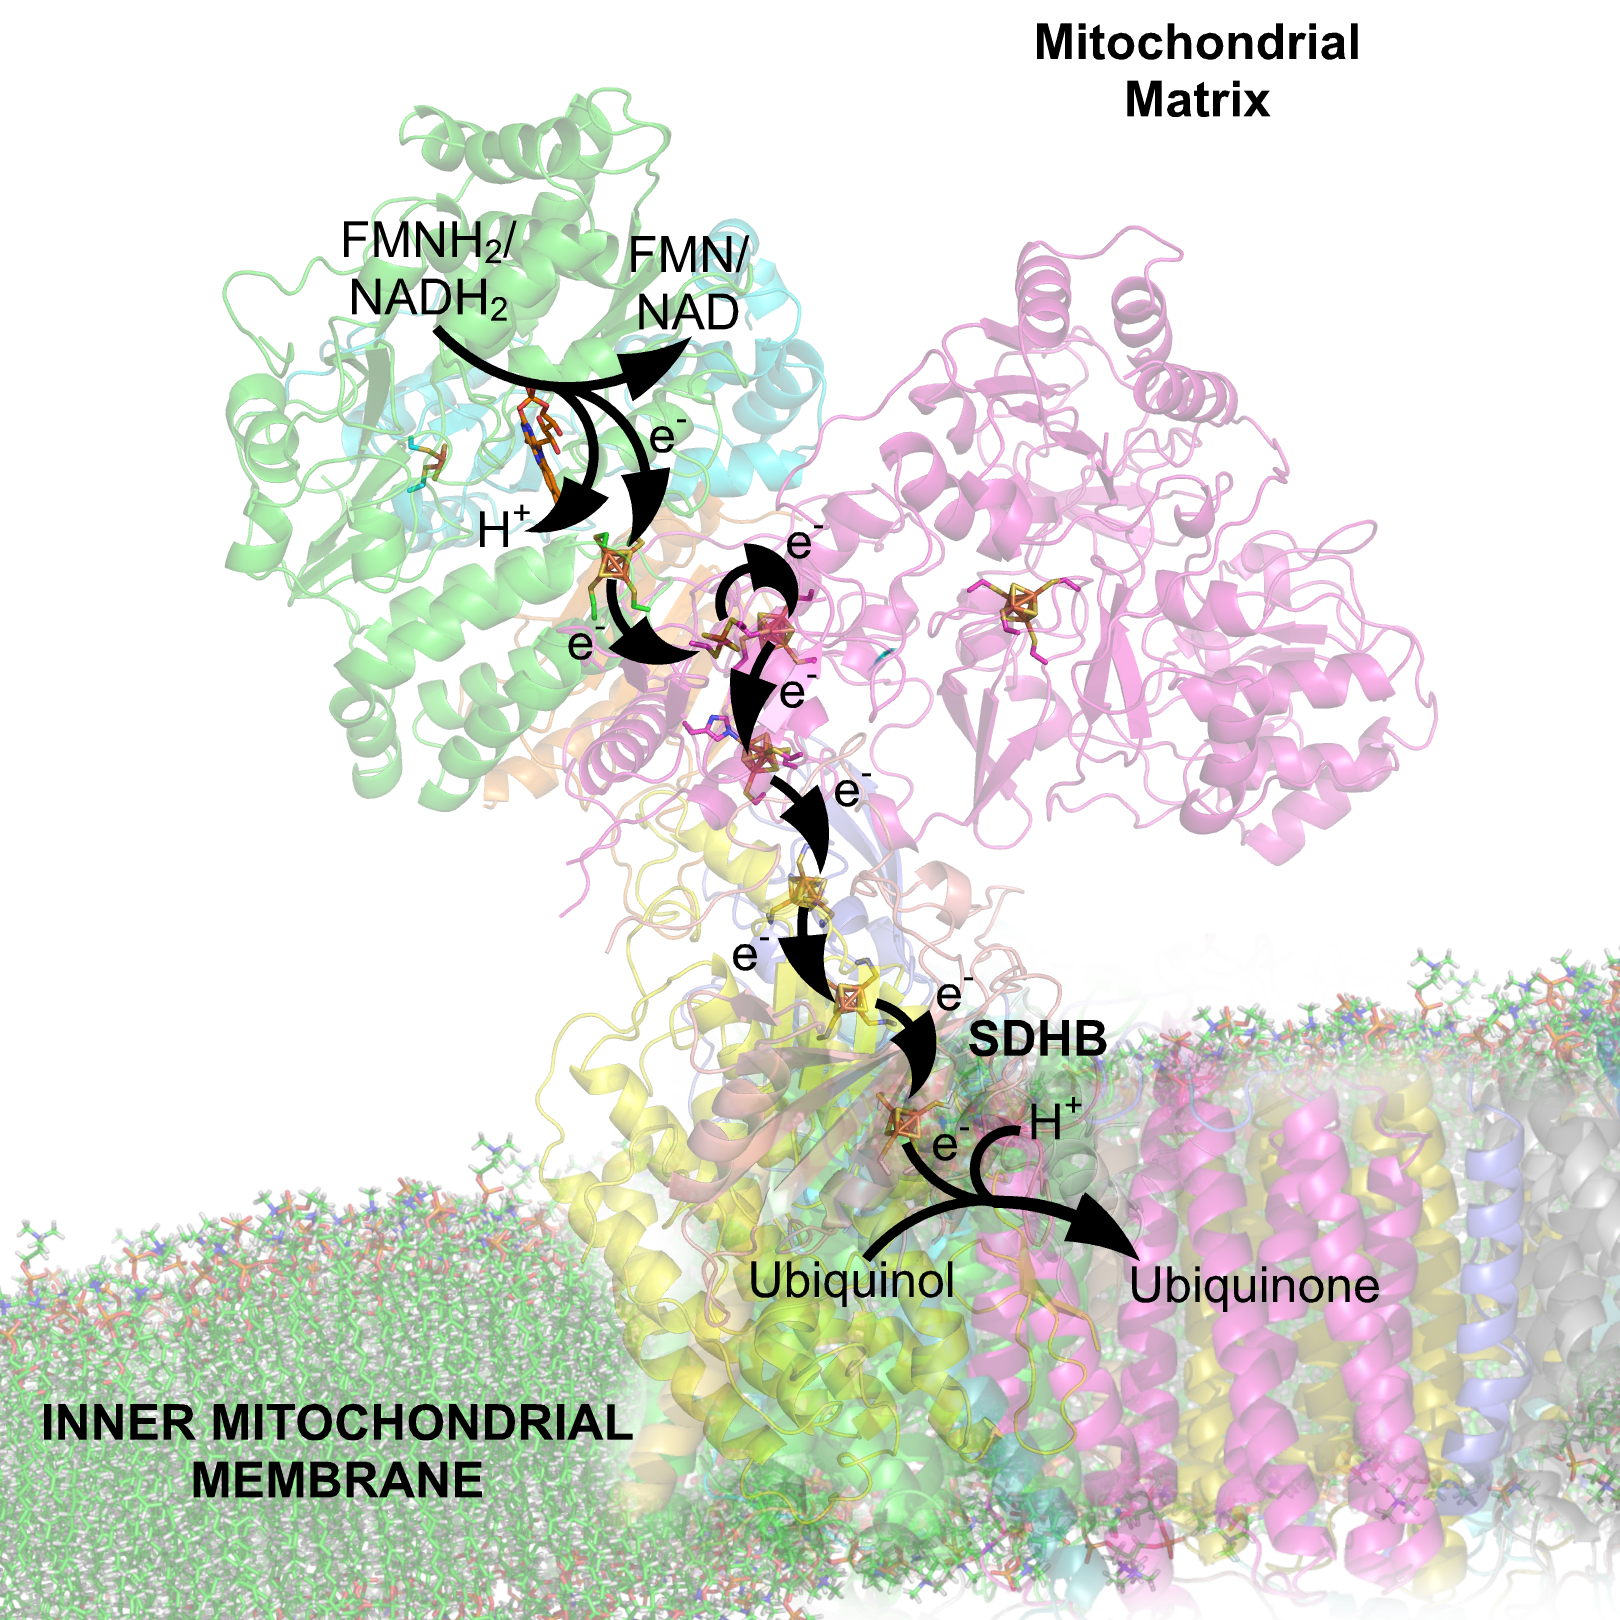
\includegraphics[width=8.5cm,height=8.5cm]{NADH.png}
	
	Fig. Proteina NADH deshidrogenasa
\end{center}


\subsection{Realizar el alineamiento múltiple de genes homólogos}
Este paso es el mas importante de todas, ya que éste establece las correspondencias posicionales en la evolución.\\
Sólo el alineamiento correcto produce inferencias filogenéticas
correctas.
\subsubsection*{Clustalo Omega}
Para el alineamiento de secuencias se utilizo el software de Clustalo Omega.
Utilizando el siguiente comando:
\begin{center}
	'clustalo.exe -i filename -o salida --outfmt=clu '
\end{center}
Donde en filename se encuentran las secuencias y salida es el archivo con las secuencias alineadas.\\


\noindent El programa \href{http://www.clustal.org/omega/}{Clustalo Omega} se encuentra tanto para windows, Linux y Mac, además se utiliza en mismo comando para realizar el alineamiento en cualquier SO.

\subsubsection*{EMBL-EBI}
En caso que no se quiera descargar el software se puede utilizar la herramiento web de EMBL-EBI \href{https://www.ebi.ac.uk/Tools/msa/muscle/}{\underline{Multiple Sequence Alignment}}.

\noindent Donde filename se enviaran a la Web, esta realizara la alineación luego se descargara los resultados en formato clustal.\\

\subsection{Modelo Evolutivo Kimura}
Ya que se quiere resultados lo más sofisticado (realista) se opto por el \textbf{Modelo Kimura}.
Este modelo considera \textbf{diferentes las tasas de mutación} para las transiciones (substitución de una purina por otra o una pirimidinas por otra) y para las transversiones (substitución de una purina por una pirimidina o vice versa).\\

De acuerdo a este modelo las transiciones ocurren más frecuentemente que las transversiones, lo cual provee mejores estimaciones de la distancia evolutiva.


\subsubsection{Construcción de la matriz de distancias}
A partir del modelo Kimura tenemos:\\
\begin{center}
	$d_{AB} = −\frac{1}{2} ln(1 − 2p_{ti} − p_{tv}) − \frac{1}{4} ln(1 − 2p_{tv})$
	
\end{center}

\noindent Donde:\\
$p_{ti}$ es la frecuencia observada de transición.\\
$p_{tv}$ es la frecuencia de transversión.\\

\noindent Las distancias evolutivas calculadas son usadas para construir una matriz de distancias entre todos los pares de taxones.

\subsection{Métodos para la construcción de árbol filogenético}	

Los algoritmos basados en distancias para construir árboles
filogenéticos pueden ser subdivididos:

\subsubsection*{Métodos basados en agrupamiento}

Los algoritmos basados en agrupamiento calculan el árbol
usando una matriz de distancias e iniciando por los pares de
secuencias más similares.

\noindent Un gran ventaja es la habilidad para hacer uso de \textbf{diferentes modelos de substitución} para corregir las distancias evolutivas.

\subsubsection*{Métodos basados en optimalidad}

Los algoritmos basados en optimalidad comparan muchas
topologías alternativas de árboles y seleccionan el que tenga el mejor ajuste entre las distancias estimadas en el árbol y las distancias evolutivas reales
\\

\noindent Los metodos basados en optimalidad requieren \textbf{mucha capacidad de computo} debido a la búsqueda exhaustiva que realizan, por ello se optó por escoger los metodos basados en agrupamiento.

\noindent El usuario podra escoger dos metodos, a partir de la interfaz grafica y seran los siguiente:
\subsubsection{UPGMA}
UPGMA (unweighted pair group method using arithmetic average)
El método más simple basado en agrupamiento.

\subsubsection{Unión de Vecinos}
El método de "Unión de vecinos" parte de una matriz de distancias, que indica la distancia entre cada par de taxones. El algoritmo comienza con un árbol completamente sin resolver, cuya topología corresponde a la de una red en estrella, y aplica los siguientes pasos hasta que el árbol está completamente resuelto y las longitudes de sus ramas.\\

\noindent Ahora que ya sabemos los pasos para la creación de arboles filogeneticos pasamos a la implementación computacional.


\section{Algoritmos e implementación computacional}
Para poder replicar el proyecto se necesitan ciertos requisitos.
\subsection{Prerrequisitos}

Los prerrequisitos son los siguientes:
\subsubsection*{Instalar Python}
Instalar python desde \href{https://www.python.org/downloads/}{\underline{Python}} para Windows o 'sudo apt-get install python3.6' para Linux.
\subsubsection*{Instalar BioPython}
BioPython es un paquete Python muy popular para manejar información biologica.
Para instalar:
\begin{itemize}
	\item conda install biopython
	\item pip install biopython
\end{itemize}

\noindent BioPython tiene tres funcionalidades principales:
Sequence Handling, 3D Structure, Population Genetics.


\noindent Antes de pasar con la implemetacion necesitamos saber con que tipo de datos vamos a trabajar, estos datos se encuentran en  archivos con terminación fasta, xml, clustal, etc. Para establecer un orden y facilidad en el mantenimiento de los algoritmos estos se encontraran en una carpeta llamada \textbf{data-gen}.

\subsection{Obtener Secuencias}
\noindent Si usted quiere replicar el proyecto con otras especies, lo unico que tiene que hacer es descargar sus secuencias en formato .fasta de NCBI y agregarlas al directorio data-gen/fasta, ver la siguiente imagen.

\begin{center}
	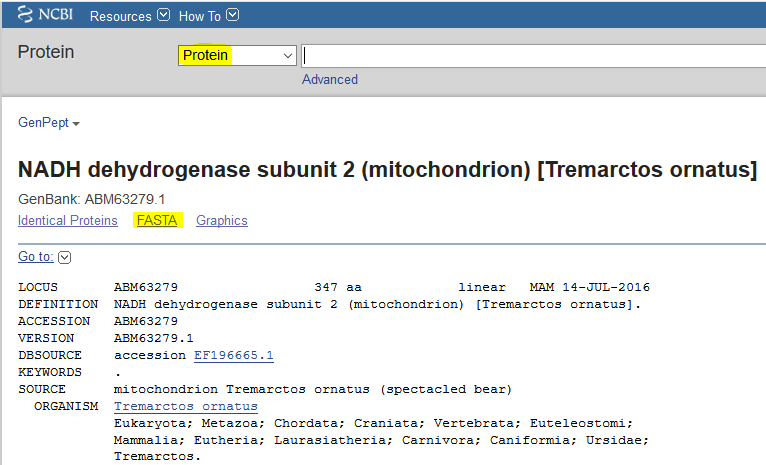
\includegraphics[width=12.5cm,height=8.5cm]{ncbi_replica.png}
	
	Fig. Descargar la secuencia .fasta haciendo click en \underline{FASTA}
\end{center}

\noindent BioPython ya tienen implementado algunos algoritmo para el manejo y alineamiento de secuencias, creacion de arboles estos nos facilitan el trabajo.

\subsection{Union de archivos fasta}

Una vez que tenemos todos nuestros archivos .fasta, pasamos a seleccionar aquellos organismos que nos interasan para su posterior análisis.

\noindent Para la selección hacemos uso de una lista llamada elegidos = [  ] que contenca los indices de las secuencias elegidas. Creamos una funcion que reciba la lista elegidos y crea un archivo en data-gen llamado \textbf{Sec-Unidas.fasta}.

\begin{center}
	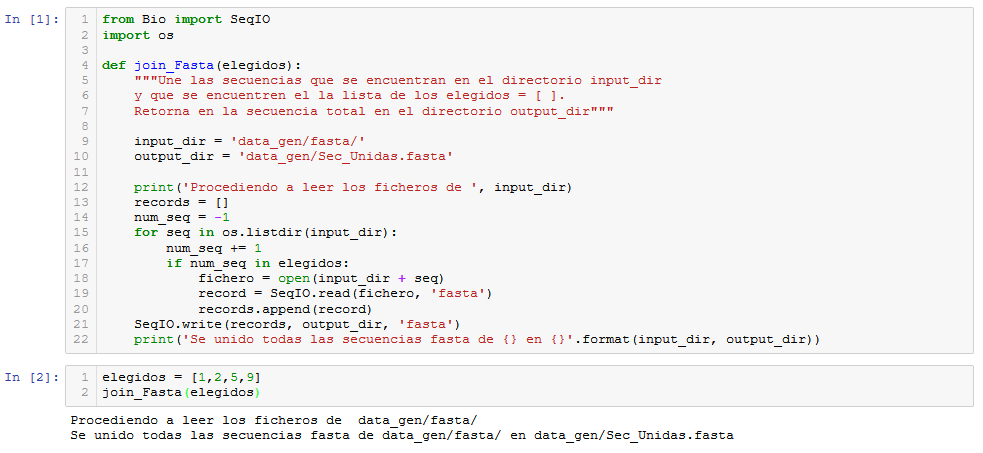
\includegraphics[width=16cm,height=9cm]{join_Fasta.png}
\end{center}

Ahora que tenemos las secuencias unidas en un solo archivo pasamos a alinearlas.

\subsection{Alineamiento de Secuencias}

\noindent Al alinear dos o más secuencias podemos observar las partes donde ellas difieren e inferir información útil sobre ellas


\noindent Un tipo de información útil es la filogenia. Esto implica que podemos inferir cómo la evolución puede explicar un conjunto particular de secuencias observadas


\subsubsection{Alineamiento Multiple}
Como se esta usando Clustalo Omega en el algoritmo se hara uso de un comando que realize el alineamiento, tambien se pueden encontrar otras herramientas revisando el REEDME que proporciana a la hora de la descarga.\\
  
\noindent El algoritmo para la implementacion recibe el archivo de las secuencias unidas y genera un archivo \textbf{.clustal} con el alineamiento, se hace uso de comandos de sistema. 
 
\begin{center}
	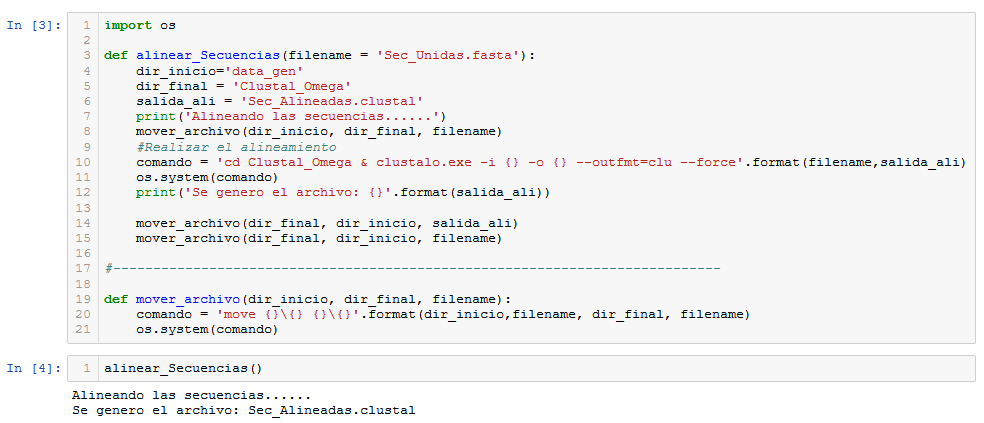
\includegraphics[width=16cm,height=6.5cm]{Alin_Sec.png}
\end{center}

\subsection{Lectura de Secuencias Alineadas}
Para poder hacer uso de las secuencias alineadas tenemos que almacenarla en una variable o tambien llamado objeto alineamiento. El siguiente algoritmo recibe la direccion del archivo clustal y retorna el objeto aligment.

\begin{center}
	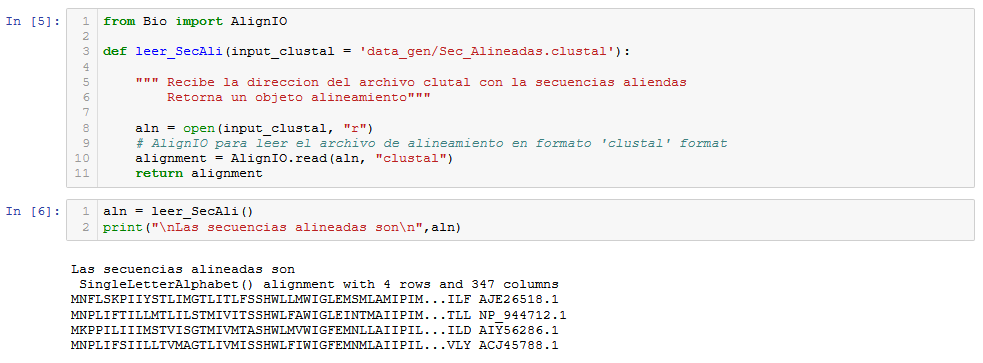
\includegraphics[width=16cm,height=7cm]{leerAlin.png}
\end{center}


\subsection{Creación de la Matriz de Distancias}
Usando el parsing del alienamiento podemos obtener la distancia (o diferencia) entre todas las secuencias.

Esto nos indica, para cada par de secuencias cuan diferentes son.
Para el caso ejemplo usamos como parametro 'identity', tambien esta el parametro 'blosum62' que toma diferentes valores de transición y transversión. 
\begin{center}
	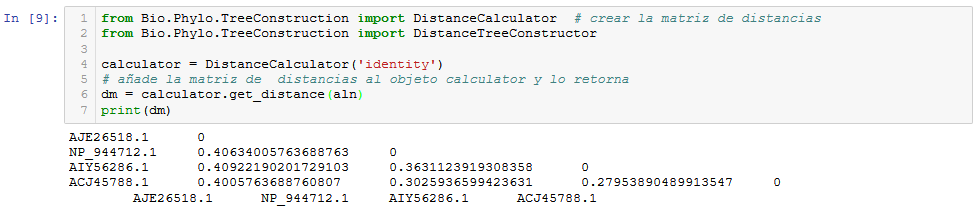
\includegraphics[width=16cm,height=4cm]{matriz.png}
\end{center}

\subsection{Creación del Arbol Filogenetico}
Finalmente, podemos construir un arbol filogenético a partir de las distancias entre todas las secuencias.
Se crea una función donde se pueda escoger el tipo de arbol a crear entre el upgma y nj(union de vecinos).

\begin{center}
	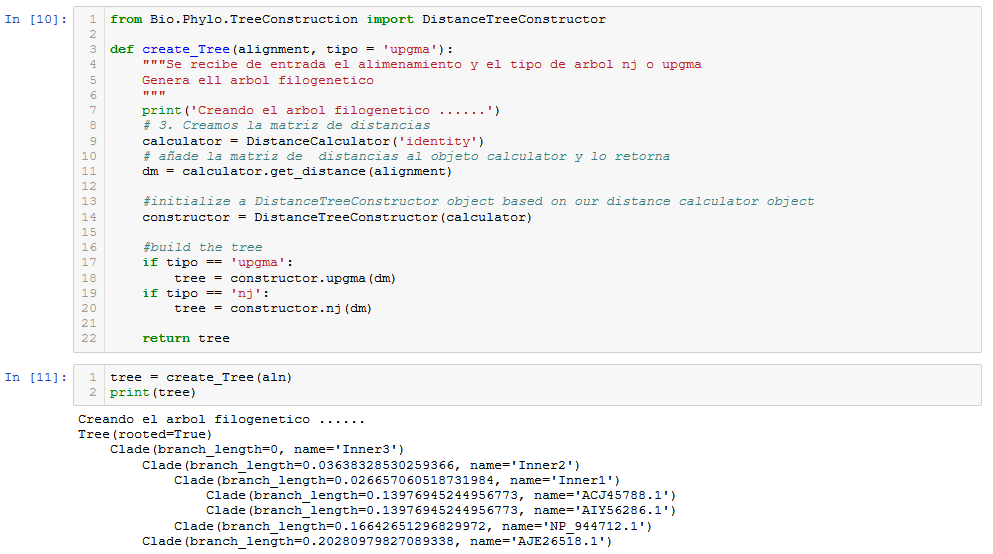
\includegraphics[width=16cm,height=10cm]{CrearArbol.png}
\end{center}
Una vez creado el objeto arbol pasamos mostrar el arbol

\subsubsection*{Mostrar Arbol}
Para mostrar el arbol usamos la funcion \textbf{Phylo.draw()}, a partir de este arbol se puede realizar el análisis.
 
\noindent 
\begin{center}
	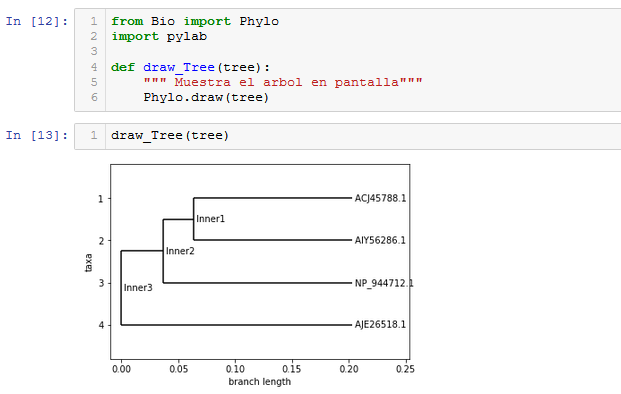
\includegraphics[width=11cm,height=5cm]{mostrarArbol.png}
\end{center}

\subsection{Modelamiento 3D de la Estrutura de Proteinas}

En las secciones pasada se utilizaron herramientas para hacer frente a las secuencias biológicas y creación de arboles filogeneticos con ´BioPython´.

\noindent El análisis de secuencia es muy importante, pero en última instancia, \textbf{la función biológica se determina por la estructura}. La gran cadena de texto(secuencia) no nos dice mucho acerca de cómo se puede hacer su función. Los biólogos estructurales son capaces de determinar lo que la secuencia se parece a cuando se toma su forma natural en la célula.

\noindent Aquí es de esa secuencia de la \href{http://www.rcsb.org/pdb/protein/O75306}{\underline{estructura}} en 3D.

Es evidente que hay mucha más información codificada en la secuencia que tenemos que considerar. Por ello solo vamos a extraer información útil a partir de esta proteína particular usando BioPython del ´PDB´ módulo.

\subsubsection{¿Qué es una estructura?}

Las biomoléculas tales como proteínas, ARN, ADN, y los productos químicos (tales como la dopamina) se componen de átomos.

\noindent Cada átomo ocupa un punto en 4 dimensiones: X, Y, Z, y el tiempo. Por ahora vamos a olvidarse del tiempo y sólo se ocupan de shapshots fijos de átomos.

\noindent Los biólogos estructurales aislar moléculas en el laboratorio, y el uso de herramientas tales como cristalografía de rayos X se puede obtener el X, Y, y Z de todos los átomos en la molécula.

\begin{center}
	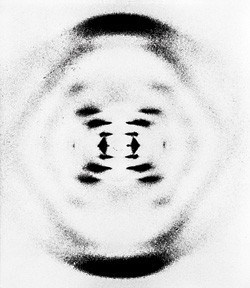
\includegraphics[width=5cm,height=5cm]{difraccion.jpg}
\end{center}

Este es el famoso patrón de difracción de rayos X de ADN utilizado por Watson y Crick y Franklin para resolver la estructura de doble hélice del ADN.

\noindent Otras tecnologías de resolución de notable estructura: microscopía electrónica, crio-microscopía electrónica, resonancia magnética nuclear (RMN).

\noindent No tenemos que preocuparnos de cómo lo hicieron, pero desde hace muchos años, estructuras resueltas (posiciones 3D de átomos de biomoléculas) se han depositado en la \href{https://www.rcsb.org/}{\underline{base de datos PDB RCSB}}.

\subsubsection{Archivo de Estructura}

\textbf{Descarga de un archivo de estructura de la base de datos PDB}

Debido a la falta de investigación de la proteina NADH deshidrogenasa en las especies endemicas elegidas, no se pudo obtener la data por ello el modelamiento 3d se realizara con el HomoSapiens \href{https://www.rcsb.org/structure/5XTB}{\underline{estructura 5XTB}}, tambien se tiene puede con otras especies como el ratón, oveja, toro, cerdo.

\begin{itemize}


\item Cada entrada en la base de datos tiene un código de identificación único.

\item El transportador de deshidrogenasa que nos interesa es: 5XTB

\item El formato del archivo principal de secuencias es \textbf{FASTA}, para las estructuras es \textbf{PDB} o \textbf{mmCIF}.

\item BioPython.PDB tiene programas de análisis para ambos.

\item \href{https://biopython.org/wiki/The_Biopython_Structural_Bioinformatics_FAQ}{\underline{Aquí}} es la página principal BioPython.PDB referencia.

\item Podemos descargar automáticamente una estructura de la base de datos utilizando el \textbf{PDBList} método del objeto \textbf{retrieve\_pdb\_file}.
	
\end{itemize}

\begin{center}
	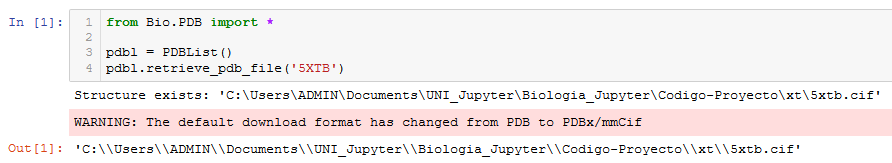
\includegraphics[width=16cm,height=3cm]{PDB.png}
\end{center}

Esa advertencia nos dice que el formato PDB es obsoleto y que el nuevo valor predeterminado es mmCIF.

Vamos a entrar en lo que parece en un poco.

Ahora deberíamos tener una carpeta que contiene 5XTB.cif en nuestro directorio de trabajo

\subsubsection{Analizar Archivos de Estructura}

Ahora vamos a extraer toda la información estructural a partir del archivo.

\begin{center}
	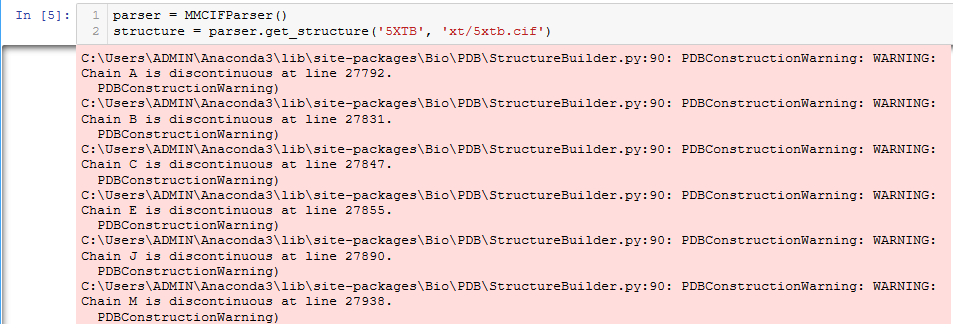
\includegraphics[width=17cm,height=6cm]{parse.png}
\end{center}

El primer argumento para el método de instancia get\_structurees un nombre opcional para la molécula, y el segundo argumento es la ruta de acceso al archivo de estructura.

Vamos a echar un vistazo a los atributos.

\begin{center}
	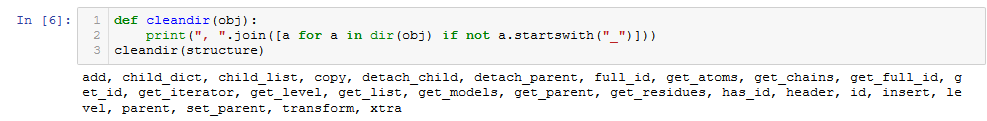
\includegraphics[width=16cm,height=2.6cm]{cleandir.png}
\end{center}

Objetos de estructura se organizan en una jerarquía específica de objetos.

\begin{center}
	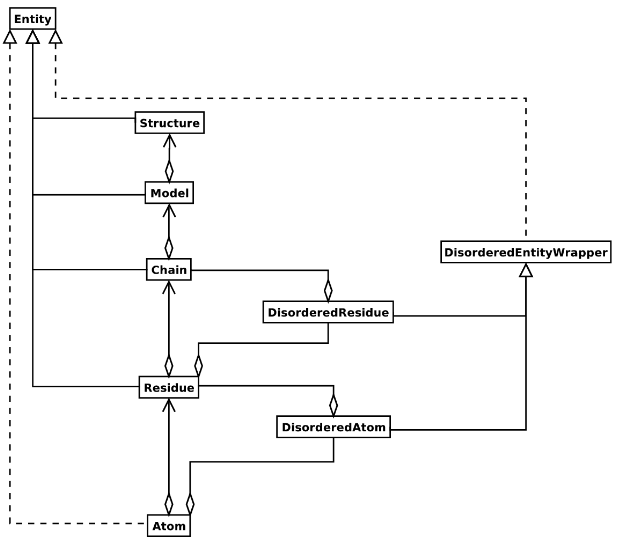
\includegraphics[width=16cm,height=8cm]{struct.png}
\end{center}

\noindent Sólo vamos a centrar en los elementos fundamentales que son: 

Modelo $\rightarrow$ Cadena $\rightarrow$ Residuos $\rightarrow$ Atom.

\begin{itemize}

\item Cada archivo de estructura puede contener varios "modelos" de la misma molécula.
\item Cada modelo contiene varios "cadenas" o hebras de proteína / ARN / ADN /.
\item Cada "cadena" se compone de residuos, o aminoácidos / bases de ADN / bases de ARN.
\item Cada residuo se compone de átomos.
	
\end{itemize}
\subsubsection{La visualización de las estructuras en Cuadernos jupyter}

Hay una muy agradable "Widget" para portátiles que nos permite visualizar objetos de estructura.

\begin{itemize}

\item conda config --add channels conda-forge
\item conda install nglview -c bioconda
\item might need: jupyter-nbextension enable nglview --py --sys-prefix

\end{itemize}
También se puede utilizar: pip install nglview

\begin{center}
	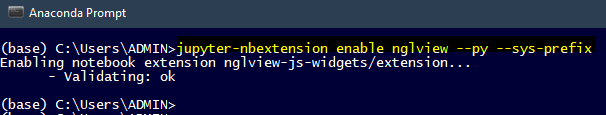
\includegraphics[width=12cm,height=2cm]{JProtein.png}
\end{center}

Para hacer manipulaciones más avanzados, es mejor utilizar herramientas independientes tales como Quimera y Pymol .\\

\noindent\textbf{Vamos a ver nuestra proteína}\\

\noindent Ahora que ya habilitamos la nglview en jupyter, desarrollamos el siguiente escript.

\begin{center}
	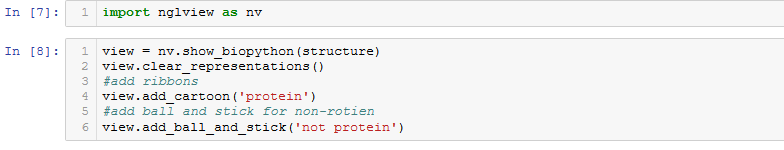
\includegraphics[width=16cm,height=3.3cm]{scriptView.png}
\end{center}

Mostramos el objeto view

\begin{center}
	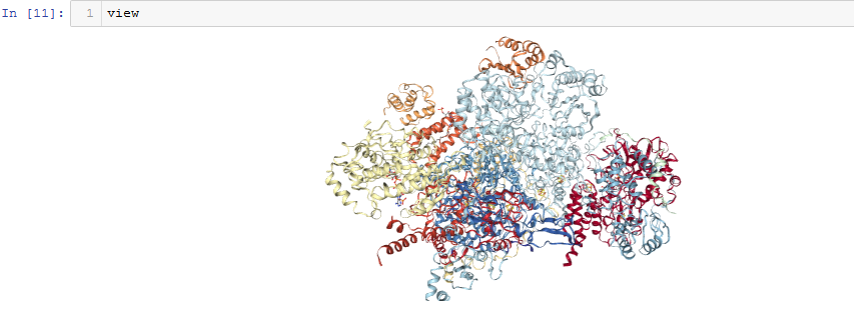
\includegraphics[width=16cm,height=6cm]{protein0.png}
\end{center}

Como era de esperar, vemos un montón cadenas donde cada cadena se visualiza como una cinta continua en el espacio 3D. Esto se conoce como una representación "cinta".

\subsection{Interfaz Gráfica}
\noindent Todos estos algoritmos y otros se encuentran como funciones en una libreria llamada \textbf{BioTool}, el cual es usado en la implementacion de la interfaz gráfica.
Para la interfaz gráfica se utiliza las siguientes librerias, estas ya vienen por defecto con python.
\begin{itemize}

\item from tkinter import *
\item from tkinter import messagebox
\item from tkinter.ttk import *
\item from PIL import Image, ImageTk

\end{itemize}
No se muestra el codigo porque posee demasiadas lineas. La intefaz final se muestra en la siguiente imagen.

\begin{center}
	
\includegraphics[width=5.5cm,height=6cm]{bienvenida.png}
	
	Fig. Ventana de bienvenida
	
\end{center}

\begin{center}
	\includegraphics[width=11cm,height=10cm]{InterfazFinal.png}
\end{center}

Donde se puede visualizar que se seleccionaron las especies, y se genero el archivo fasta, con la unión de todas las secuencias de proteina de las especies elegidas.

El boton seq genera una ventana con la información de la secuencia buscador de nucleotidos por posicion y por bloqes para el análisis.

\begin{center}
	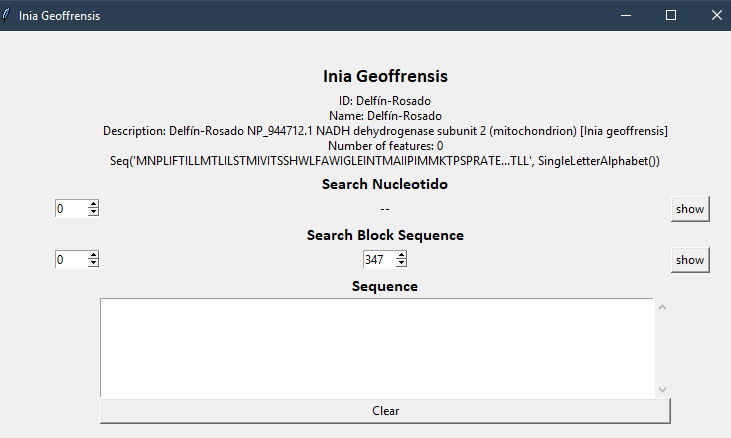
\includegraphics[width=15cm,height=8cm]{boton-seq.png}
\end{center}

El boton info muestra inforamción de la especie, tales como el nombre común, ubicación de la especie, Taxonomia, Estado de conservación.

\begin{center}
	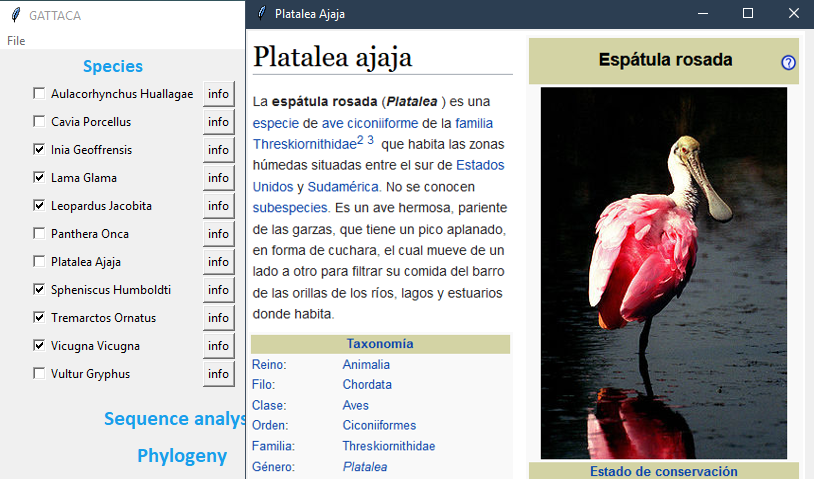
\includegraphics[width=17cm,height=10cm]{info.png}
\end{center}

El boton multiple, genera el alineamiento multiple de las secuencias, genera una ventana con el alineamiento.

\begin{center}
	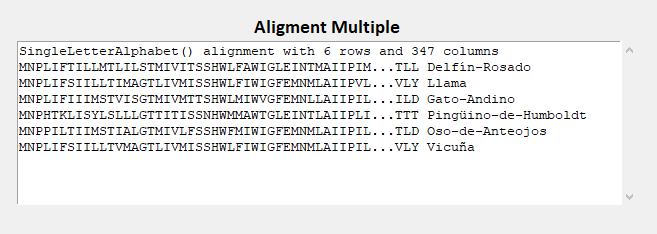
\includegraphics[width=12cm,height=4cm]{multiple.png}
\end{center}


\section{Resultados}
Una descripción de los resultados [esperados en el caso de la propuesta]. Un reporte integrando los resultados proporcionados por la herramienta

\subsection{Verificar la fiabilidad del árbol construido}
Para la fase beta se encontró el siguiente árbol.

\begin{center}
	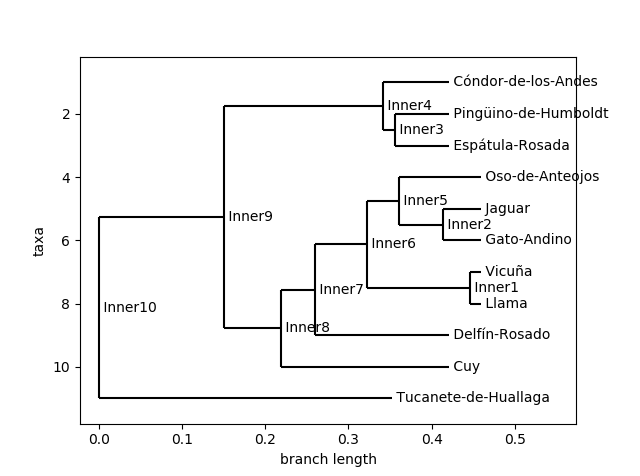
\includegraphics[width=12.5cm,height=8.5cm]{arbol.png}
	
	Fig. Árbol utilizando el método UPGMA
\end{center}

\subsection{Análizar el árbol filogenético}
Para diferentes métodos son diferentes los árboles generados. Es importante escoger la misma proteína para todas las especies.

Sin embargo, es importante notar que, en ambos árboles, los mamíferos se encuentran más cerca de los mamíferos y los oviparos más cerca de los mamíferos. Además, dentro del grupo de los mamíferos, los felinos muestran estár más cerca entre ellos. Un caso similar a ello es el de los auquénidos.

\begin{center}
	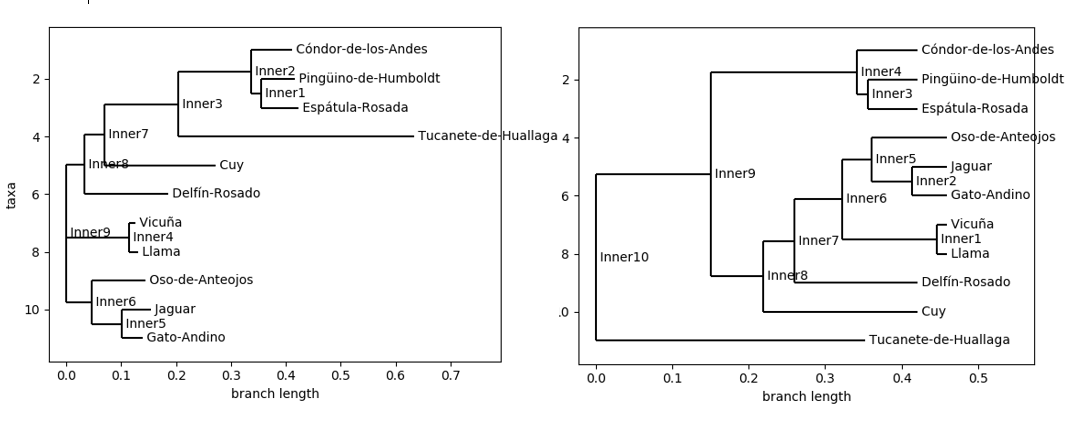
\includegraphics[width=15.5cm,height=8.5cm]{tree_comparation.png}
	
	Fig. Comparación entre árboles UPGMA y Neighbor
\end{center}
\subsubsection{Modelamiento 3D de la Proteina}

\noindent\textbf{Representación cinta}\\

\noindent Podemos ver que tenemos 5 cadenas diferentes de color rojo, azul, celeste, naranja, crema.
\begin{center}
	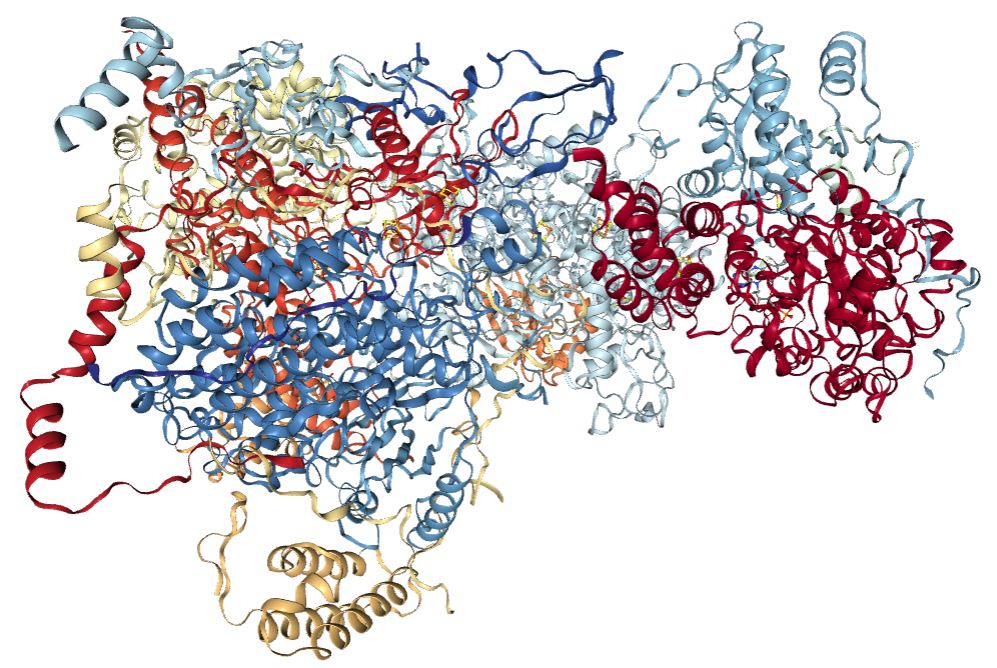
\includegraphics[width=16cm,height=12cm]{protein1.png}
	
	Fig. Modelo 3D de la proteina NADH deshidrogenasa en el HomoSapiens 
\end{center}

\noindent\textbf{Ligando}

Ligando a aquella molécula que se une al centro activo de la proteína para que ésta pueda realizar su función (transportar, o inhibir una reacción metabólica).

Además existen varios tipos de ligandos.

\begin{center}
	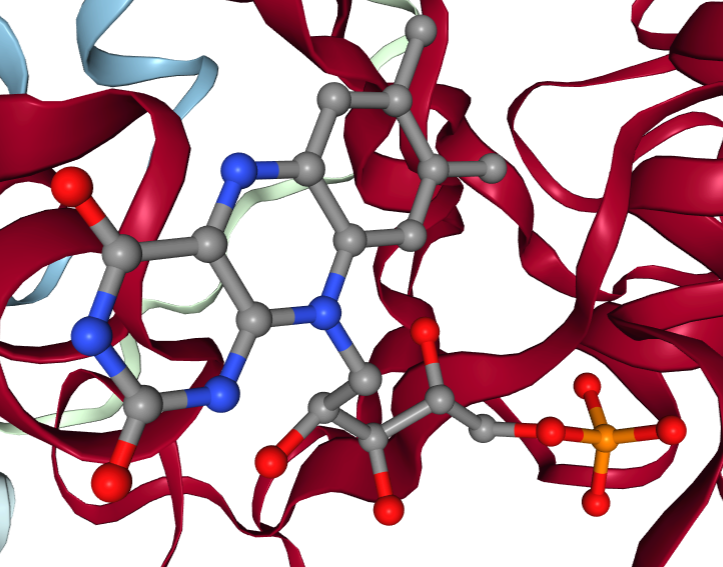
\includegraphics[width=6cm,height=4cm]{ligando1.png}
	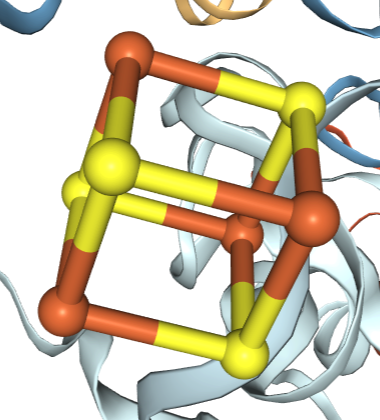
\includegraphics[width=4cm,height=4cm]{ligando4.png}
		
\end{center}


\begin{center}
	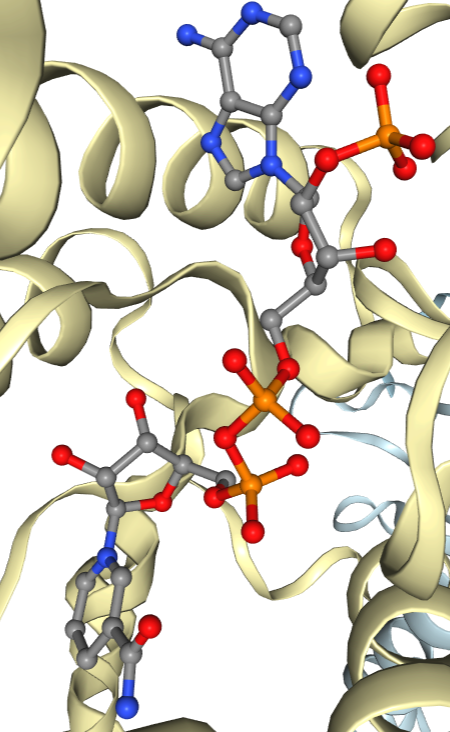
\includegraphics[width=5cm,height=7cm]{ligando2.png}
	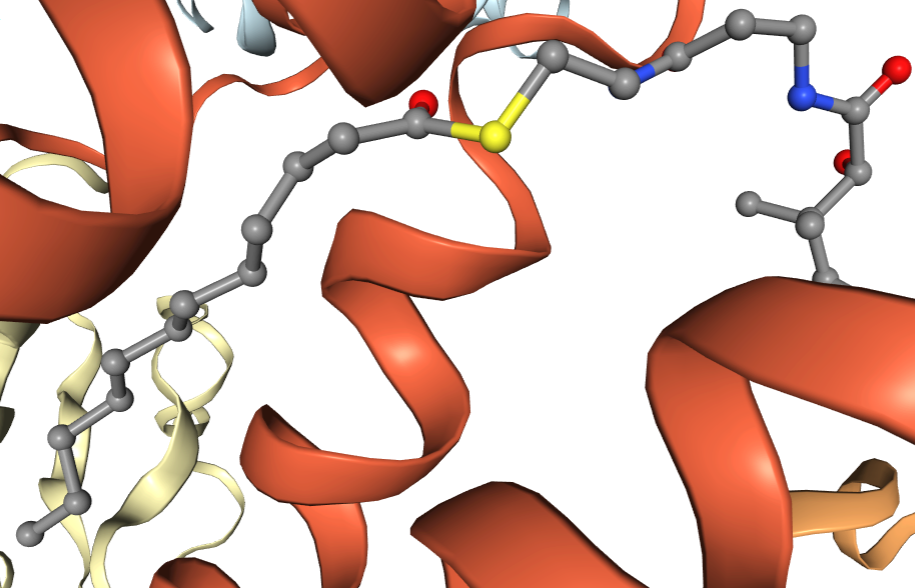
\includegraphics[width=4cm,height=6cm]{ligando3.png}
	
\end{center}

\section{Conclusiones}

El presente proyecto llamado GATTACA consistió en crear un programa con interfaz gráfica que muestra cómo utilizar los recursos informáticos de BioPython para el alineamiento múltiple de secuencias y creación de árboles filogenéticos para especies endémicas. Dentro de las ventajas el usuario puede escoger aquellas especies que quiere analizar, en caso de querer analizar otras especies solo necesita seguir los pasos de la implementación y poner su data en algunos directorios, también se puede replicar el modelamiento 3D. Entre las desventajas se tienen que el programa requiere la instalación de varias librerías y paquetes de Python y Bio. Para los trabajos futuros se pretende poder realizar un modelamiento 3D con animación.

\begin{thebibliography}{0}
	
	\bibitem{} Biopython\\ \textcolor{blue}{\url{https://biopython.org/}}.
	
	\bibitem{}The Biopython Structural Bioinformatics FAQ\\
	\textcolor{blue}{\url{https://biopython.org/wiki/The_Biopython_Structural_Bioinformatics_FAQ}}.
	
	\bibitem{}Construcción de arboles filogeneticos apartir de base de datos geneticos\\ \textcolor{blue}{\url{https://www.researchgate.net/publication/316217579_BIOINFORMATICA_EN_EL_AULA_CONSTRUCCION_DE_ARBOLES_FILOGENETICOS_A_PARTIR_DE_BASES_DE_DATOS_MOLECULARES}}.
	
	\bibitem{}Realizar el árbol filogenético\\ \textcolor{blue}{\url{http://elviajedelnavegante.blogspot.com/2015/05/generacion-de-arboles-filogeneticos.html}}.
	
	\bibitem{} Modelado de la proteina\\ \textcolor{blue}{\url{https://eead-csic-compbio.github.io/bioinformatica_estructural/node35.html}}.
	
	
	
	
\end{thebibliography}



\end{document}